\documentclass[tikz]{standalone}
\usetikzlibrary{positioning}
% newcommands.tex

\newcommand{\enq}{\texttt{enq}}
\newcommand{\deq}{\texttt{deq}}
\newcommand{\pput}{\texttt{PUT}}
\newcommand{\get}{\texttt{GET}}
\newcommand{\vs}{\texttt{vis}}
\newcommand{\so}{\texttt{so}}
\newcommand{\arb}{\texttt{ar}}
\newcommand{\rf}{\texttt{rf}}

% example
\newcommand{\po}[2]{\draw [->, thick] (#1) to node[above] {\Large{\so}} (#2);}
\newcommand{\pva}[2]{\draw [->, thick] (#1) to node[above] {$\Large{\so},\Large{\vs},\Large{\arb}$} (#2);}
\newcommand{\pbva}[2]{\draw [->, thick] (#1) to node[above] {$\Large{\so}$} node[below] {$\Large{\vs},\Large{\arb}$} (#2);}
\newcommand{\pv}[2]{\draw [->, thick] (#1) to node[above] {\Large{\so}} node[below] {\Large{\vs}} (#2);}
\newcommand{\evis}[2]{\draw [->, thick] (#1) to node[above, sloped, near end] {\Large{\vs}} (#2);}
\newcommand{\mvis}[2]{\draw [->, thick] (#1) to node[above, sloped] {\Large{\vs}} (#2);}
\newcommand{\ar}[2]{\draw [->, thick, allow upside down] (#1) to node[above, sloped] {\Large{\arb}} (#2);}
\newcommand{\va}[2]{\draw [->, thick, allow upside down] (#1) to node[above, sloped] {$\Large{\vs},\Large{\arb}$} (#2);}
\newcommand{\vab}[2]{\draw [->, thick, allow upside down] (#1) to node[below, sloped, near end] {$\Large{\vs},\Large{\arb}$} (#2);}
\newcommand{\vae}[2]{\draw [->, thick, allow upside down] (#1) to node[above, sloped, near end] {$\Large{\vs},\Large{\arb}$} (#2);}
\newcommand{\vas}[2]{\draw [->, thick, allow upside down] (#1) to node[sloped, near start, above] {$\Large{\vs},\Large{\arb}$} (#2);}

% serialization
\newcommand{\scc}[2]{\draw [->, very thick] (#1) to (#2);}
\newcommand{\rva}[2]{\draw [->, thick, allow upside down] (#1) to node[above, sloped] {$\Large{\rf},\Large{\vs},\Large{\arb}$} (#2);}
\newcommand{\rvb}[2]{\draw [->, thick, allow upside down] (#1) to node[below, sloped] {$\Large{\rf},\Large{\vs},\Large{\arb}$} (#2);}


\renewcommand{\va}[2]{\draw [->, thick] (#1) to (#2);}

\begin{document}
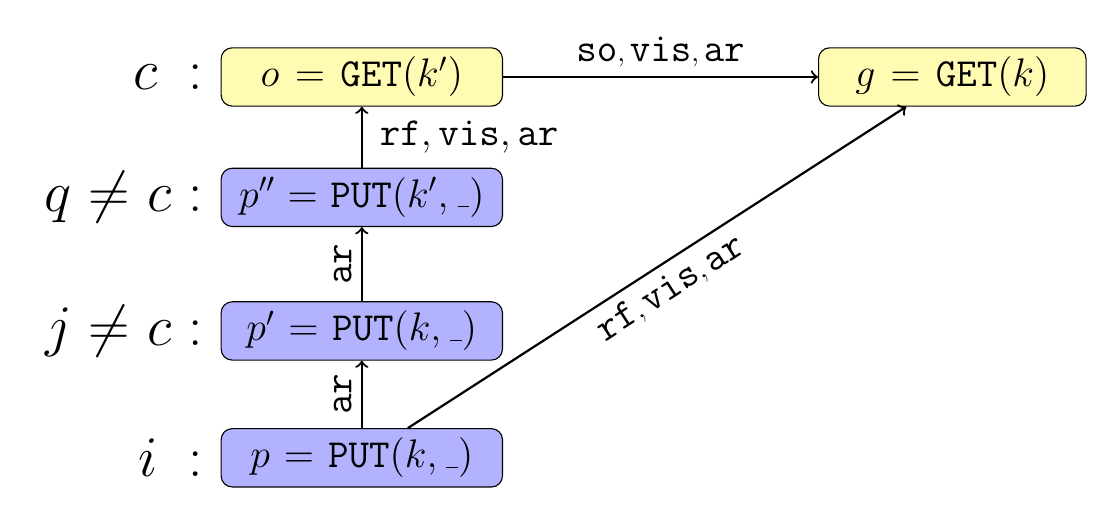
\begin{tikzpicture}
\tikzset{
 process/.style = {rectangle, font = \huge, text width=6em, align = right},
 put/.style = {rectangle, rounded corners,font =\Large, fill = blue!30, draw, text width=9.5em, text centered},
 get/.style = {rectangle, rounded corners,font =\Large, fill = yellow!30, draw, text width=9.5em, text centered},
 g/.style = {rectangle, font =\Large, rounded corners,draw, fill = yellow!30,text width=9em, text centered},
 vis/.style = {rectangle, font = \Large}
}
  \node (p-c) [process] {$c:$};
  \node (o) [get, right = 0.1cm of p-c] {$o=\get(k')$};
  \node (g) [g, right = 4.0cm of o] {$g = \get(k)$};

  \node (p-q) [process, below = 0.8cm of p-c] {$q \neq c:$};
  \node (p'') [put, right = 0.1cm of p-q] {$p''=\pput(k',\_)$};

  \node (p-j) [process, below = 0.8cm of p-q] {$j\neq c:$};
  \node (p') [put, right = 0.1cm of p-j] {$p'=\pput(k,\_)$};

  \node (p-i) [process, below = 0.8cm of p-j] {$i:$};
  \node (p) [put, right = 0.1cm of p-i] {$p=\pput(k,\_)$};

  \pva{o}{g};

  \ar{p}{p'};
  \ar{p'}{p''};

  \rvb{p}{g};
  \va{p''}{o};
  \node [vis, below right = 0.15cm and 2cm of p-c] {$\Large{\rf},\Large{\vs},\Large{\arb}$};
\end{tikzpicture}
\end{document}
